\documentclass{llncs}
\usepackage[latin1,utf8x]{inputenc}
\usepackage{color}
\usepackage[pdftex]{graphicx}
\usepackage{amsmath}
\usepackage{verbatim}
\usepackage{marginnote} 

\newcommand\margin[1]{\marginnote{\scriptsize{\bfseries #1}}}



\title{Classification Techniques for Conformance and Performance Checking in Process Analysis}
\author{Hind Chfouka\inst{1}, Andrea Corradini\inst{1} and Roberto Guanciale\inst{2}}
\institute{Department of Computer Science, University of Pisa, Italy \\ 
\email{\{chfouka,andrea\}@di.unipi.it}\and School of Computer Science and Communication,
KTH Royal Institute of Technology, Stockholm, Sweden \\
\email{robertog@kth.se}}	
\date{today}

\begin{document}
\maketitle
\begin{abstract}
Standard process analysis techniques, like conformance checking or performance evaluation, are enabled by the existence of event logs that trace the process executions and by the presence of a model that formally represents the process. Such analysis techniques use only part of the huge amount of data recorded in event logs. In this paper the goal is to exploit this data to extract useful information for  conformance checking and  performance analysis. We present an approach that using standard classification technique, explores how data influence process behaviors by affecting its conformance or performance.
\end{abstract}

\section{Introduction}
Today, many Information Systems that support  the concept of business process record all events occurring during the process execution in  event logs. An event log represents a trace of the process behavior that can be observed and analyzed in order to tune it with the business objectives pursued. Process Mining provides a set of techniques for process discovery and analysis. Through the knowledge extracted from event logs, process discovery allows one to construct a process model. Process analysis instead assumes the existence of a model and it consists of checking the conformance and performance of the process executions with respect to it.

The work presented in this paper is motivated by the observation that existing event logs are rich of data, but such data is used only in part by the existing process analysis techniques. Since data is considered as a valid source of knowledge, developing techniques based on data analysis can provide advantages for  process discovery and analysis.
This fact has already been observed several times in the literature, and it brought to the development of various approaches where machine learning techniques are applied to workflow or process discovery (see e.g.~\cite{DBLP:conf/ecml/Herbst00,Maruster-PHD,DBLP:conf/bpm/RozinatA06,DBLP:conf/sac/LeoniA13}).

Here instead, we consider more specifically process analysis. Our goal is to find a way to transform the data recorded during the process activities in knowledge useful for the analysis.  In particular,  we try to determine how data may affect the conformance and performance of process executions. Identifying this influence can provide qualitative information about the causes of possible anomalies in the process behaviors, facilitating the task of taking corrective measures.

In order to analyze data contained in event logs, we propose an approach based on {machine learning}~\cite{tan2005introduction}, where we exploit \emph{classification} techniques to find patterns on data in presence of which conformance errors occur. The same approach has been extended to evaluate how data influences  process efficiency, by combining classification problems with performance evaluation: this is just summarized briefly in the paper due to size constraints.  Classification is a well-known {machine learning} technique which consists of identifying to which category, among a given set, a new observation belongs. This is done on the basis of a training set of data containing observations whose category membership is known.

After the presentation of a case study in Section~\ref{example}, Section~\ref{Background} introduces some background concepts about process analysis. First the log replay algorithm is briefly described, then conformance  analysis is introduced using the business process of Section~\ref{example}. In Section~\ref{ClassifApproach} our approach to process analysis based on classification is presented. First a few basic concepts about the classification technique are described, next the conformance analysis based on classification is presented in detail through an illustration with our case study.  A possible extension of the approach for performance analysis is briefly discussed presented. Finally, Section~\ref{implementation} describes the implementation of our approach provided as \emph{ProM6}\cite{DBLP:conf/bpm/AalstDGRVW09} plug-ins, as well the methodology to follow in order to analyse processes using our approach.

\section{The Case Study: a Sale Business Process}\label{example}
A business process can be seen as a collection of activities occurring within an organization that lead to a specific goal. There are several formalisms for representing business processes. In this paper we represent them using Petri nets~\cite{DBLP:conf/ifip/Petri62,DBLP:journals/jcsc/Aalst98} since this makes possible to exploit some existing process analysis techniques that are based on such nets. However, in a business management context, Petri nets can be not expressive enough and usually process models are presented as workflows, for example using a standard notation for the business process modeling: BPMN (Business Process Model and Notation)~\cite{BPMN}. Transforming a BPMN model into a Petri net is possible thanks to a mapping technique presented in~\cite{DBLP:conf/wsfm/BruniCFFGS11}.
\begin{figure}[h]
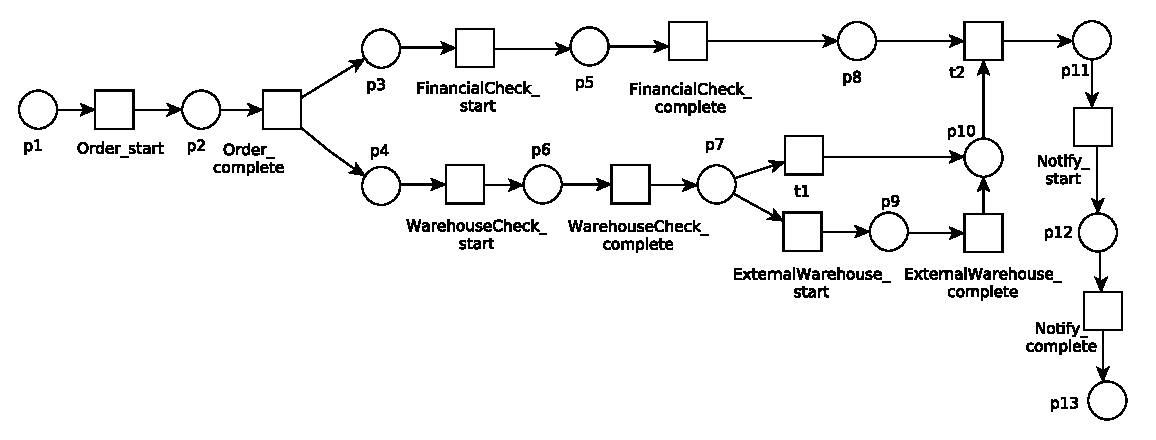
\includegraphics[width=360pt]
{./items/Sales_PN.pdf}
\caption{Petri net for a sale process}
\label{pnet}
\end{figure}
%
Figure~\ref{pnet} presents the Petri net model for a sale
process.\footnote{\small{
The Petri net of Figure~\ref{pnet} is obtained by
transforming a BPMN model using the algorithm of~\cite{DBLP:conf/wsfm/BruniCFFGS11}, and mapping
each activity to a pair of start/end transitions. The resulting net
has been simplified by removing the unnecessary \emph{invisible
  transitions} used to encode the \emph{Join} or \emph{Fork} gateway~\cite{DBLP:conf/wsfm/BruniCFFGS11}.
}} 
This business process abstractly represents a fragment of the procedure followed in a commercial organization for managing orders received from clients. In general this procedure includes several activities and each of them involves a specific department of the organization. We assume that the sale process begins with the notification of an order from a client, so the first activity is simply called \emph{Order}. After the order is received, the sale process continues with some activities that can be done in parallel, since they do not present any dependency. The \emph{FinancialCheck} activity represents the financial analysis of the order (i.e verifying the financial situation of the client). Concurrently, the \emph{WarehouseCheck} activity checks the availability of merchandise requested by the order and, in case of a shortage, starts a supplying procedure. This is done through the activity \emph{ExternalWarehouse}. After the completion of the  parallel activities, a synchronization is needed before continuing the sale procedure with the final activity called \emph{Notify}, by which a result regarding the acceptance of the order is communicated to the client.

\section{Process Analysis}\label{Background}
Process analysis is performed using the Petri net representing the process and an event log recording the related executions, also called \emph{process instances}. The basic building blocks of event logs are \emph{events}, that record the execution of the process actions. Therefore an event $e$ can be seen as a tuple including the action recorded, a corresponding timestamp, and possibly other attributes describing relevant information about the state of the process. Events that belong to the same process instance are grouped in a {\itshape trace}, where events are ordered  by timestamp. An \emph{event log} is a set of traces, recording the activities performed by a system during a finite number of process executions.  In this paper the following assumptions are made:
\begin{itemize}
\item All traces are instances of the same process.
\item For each action there exists a corresponding transition in the net that will be denoted, for simplicity, by the same name of the action.
\end{itemize}

\subsection{Log replay algorithm}\label{logreplayAlg}
The key algorithm exploited to analyze a Petri net model with respect to an event log is the {\itshape log replay} algorithm (see e.g.~\cite{DBLP:journals/is/RozinatA08}). Given a Petri net model and an event log as input to the algorithm, for each trace in the log, the algorithm starts by placing one token in the start place of the net. For each event in the trace the corresponding transition is fired assuming a  non-blocking behavior, then the marking of the net is updated. \emph{Non-blocking replay} means that whenever a firing of a disabled transition is needed, the algorithm enables the transition either by creating artificial tokens in the pre-set or, if possible, by firing some invisible transitions; the non-determinism in this procedure is resolved with a suitable cost function. For each trace, the result of the log replay execution is a map indicating which transitions of the model have been fired for each event in the trace, and additionally which tokens were artificially created and which remained  upon completion of the trace. The output of the log replay algorithm  can be used to check the conformance of the traces.

\subsection{Conformance Analysis}\label{ConformanceAnalysis}
The goal of the conformance analysis is to check if a trace complies with the Petri net modeling the business process. Conformance problems can be discovered by analyzing tokens artificially created during the replay {\itshape (the missing tokens)} and tokens not consumed {\itshape (the remaining tokens)}. Figure~\ref{ConfLog}  presents two different traces, $T$ and $T'$, of the business process presented in Section~\ref{example}, where only the actions and the timestamps are reported. The log replay of trace $T$, which is compliant with the Petri net, terminates with a single remaining token in the end place \{${p13 \rightarrow 1}$\} and without reporting  missing tokens.

\begin{comment}
\begin{equation}
\begin{split}
R&=\{(Order\_start,1), (Order\_complete,2),(WarehouseCheck\_start,3), \\
& (FinancialCheck\_start,4),(FinancialCheck\_complete,5),\\
& (WarehouseCheck\_complete,6),(t2, 7), (Notify\_start,7), \\
&(Notify\_complete,8)\}
\end{split}
\end{equation}
\end{comment}

\begin{figure}[h]
\centering
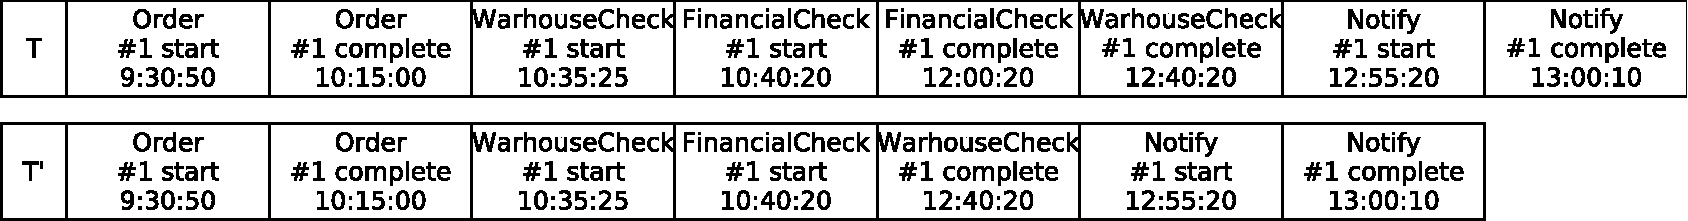
\includegraphics[width=345pt]
{./items/logConforme.pdf}
\caption{Conforming ($T$) and non-conforming ($T'$) traces}
\label{ConfLog}
\end{figure}

The log replay of the trace $T'$ terminates with remaining tokens \{$p5 \rightarrow 1$, $p13 \rightarrow 1$\} and one missing token \{${p8 \rightarrow 1}$\}. The missing token is created artificially and this fact witnesses a wrong execution of the event \emph{Notify\_start}. In fact, in $T'$ this event is executed before the termination of the activity \emph{FinancialCheck}: this is interpreted as a non-conformance to the process model. 

\section{Classification for Process Analysis}\label{ClassifApproach}
Exploiting machine learning techniques for process analysis is encouraged by the presence of a huge amount of data recorded as attributes in event logs. The implicit information contained in those data could be significant for the process behavior analysis. In fact, this potential information could contain an explanation for the deviations discovered during conformance analysis, and for the performance level provided by the process. For this reason, we are interested in discovering how the process data may influence the conformance and the performance of the process executions. This is done with an approach based on \emph{classification}, a classical machine learning technique able to detect patterns on data in correspondence to which the process assumes a specific behavior.

\subsection{Classification: Basic Concepts}\label{classifBasicConcept}

In a classification problem~\cite{tan2005introduction}, data is represented by a collection of records (called instances), and each of them is characterized by a tuple $(\mathbf{x},y)$, where $\mathbf{x}$ is a set of attributes and $y$ is a special one called \emph{target attribute}. The value of the target attribute is a label identifying   the class to which the record belongs. The goal is to learn a classification model that maps each attribute set $\mathbf{x}$ to one of the predefined class labels $y$.

The general approach for solving a classification problem~\cite{tan2005introduction} consists of providing a \emph{training set} of records, whose class labels are already known, to the learning algorithm in order to build a classification model. This model is then applied to a \emph{test set}, which consists of records with unknown class labels. This step allows to  estimate the \emph{model accuracy} using one of the standard approaches. For example, the accuracy can be represented by the percentage  of records correctly predicted  with respect to the total number of records in the test set.

Many classification models can be applied to a classification problem. For our purpose we choose the \emph{decision tree} model since the rules detected by the classification are shown explicitly, providing an overview of how process data affects the process behavior. In a decision tree, a class label (possible value of the target attribute) is assigned to each leaf node. The non-terminal nodes, which include the root and the internal nodes, contain attribute test conditions to filter records that have different characteristics.

\subsection{Classification for Conformance Checking}\label{ClassConformance}
In order to identify the possible causes of non-conformance, a classification problem can be formulated. The classification dataset is extracted from the process data: for each process instance, relevant information is  extracted and included as a record in the dataset. For the process presented in Section~\ref{example}, a record includes  the following attributes: an instance identifier, a  client identifier, the client typology (new or consolidated client), the sales manager responsible for the order, the financial officer who conducts the financial evaluation activities, the warehouseman responsible for the warehouse checking, the supplying responsible name in case of a provision, and finally the result communicated to the client for the order issued. Furthemore, as target attribute we associate with each record the conformance result for that instance,  which is a boolean value that is extracted from the output of the log replay. All these attributes are discrete and contribute to build the dataset
presented in Table~\ref{tab:SaleData} of the classification problem. In this preliminary work,  in order to 
explore the applicability of existing machine learning  techniques to process analysis, we just used synthetic data
generated to emulate process executions. Note that for this  running example, attributes selected for the classification task are all focused on the actors of the process activities. In general, an attribute can characterize several aspects of an activity.

In order to build the classification problem, the attributes characterizing the process are extracted from the log, while the conformance attribute is computed using the conformance checking algorithm. The Petri net of Figure~\ref{replayResult}  shows the output of the conformance analysis executed on the event log: edges are labeled with the number of times they were activated, places are labeled with the number of remaining and missing tokens.

\begin{figure}[h]
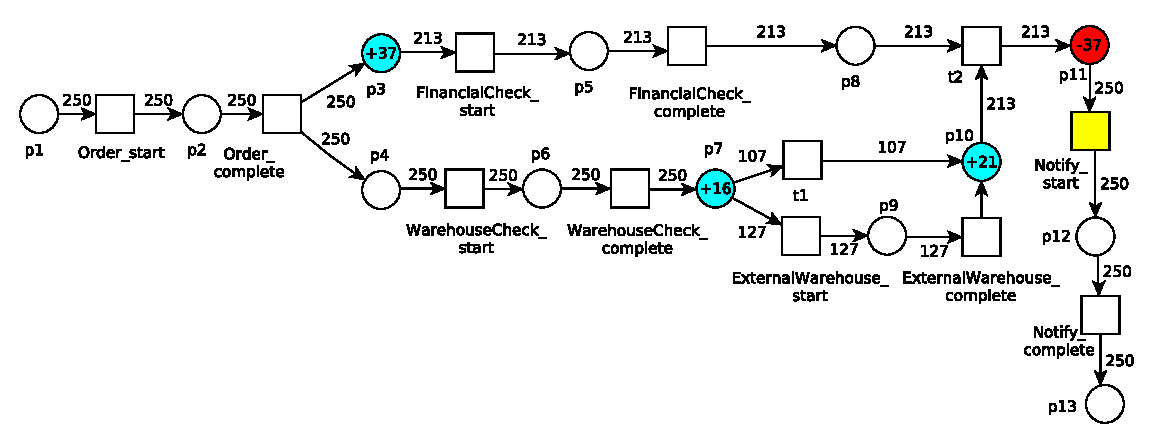
\includegraphics[width=360pt]
{./items/Sales_PN_resultMod.pdf}
\caption{Petri net: conformance results.}
\label{replayResult}
\end{figure}

The resulting data highlight  that there are 37 out of 250 process executions with conformance errors. The presence of 37 missing tokens in $p11$ represents  the number of times that the log replay  algorithm forced the execution of transition \emph{Notify\_start}, even if it was not enabled, in order to mimic a corresponding event in the trace.

Moreover, 37 remaining tokens in place $p3$ indicate the number of
times that the financial check activities were not performed.
Taking into account the application scenario, we can conclude that 
37 instances of the process are not compliant with the sale policy since
they did not execute the financial check activity.
{
\renewcommand{\arraystretch}{1.2}
\begin{table}[!h]
\scriptsize{
\caption{Dataset for the conformance analysis.}

\begin{tabular}{|p{1cm}|p{1cm}|p{1,5cm}|p{1,3cm}|p{1,3cm}|p{1,2cm}|p{1,5cm}|p{1,4cm}|p{0,8cm}|}
\hline OrdIde & CltIde & CltType & SalMan & FinOff & WrhsMan & SupplyResp & OrdResut & Conf\\
\hline
1 & 20 & consolidate & Marco & Mary & Alex & Gianni & positive & no\\
\hline
2 & 15 & new & Anna & Johann & Roberto & Mario & positive & yes\\
\hline
3 & 10 &consolidate & Maria & Mary & Alessio & Gianni & negative & no\\
\hline
10 & 18 & consolidate & Johann & Mary & Roberto & Gianni & positive & yes \\
\hline
... & ... & ... & ... & ... & ... & ... & .... & ...  \\
\hline
\end{tabular}
}
\label{tab:SaleData}
\end{table}
\normalsize


\begin{figure}[h]
\centering
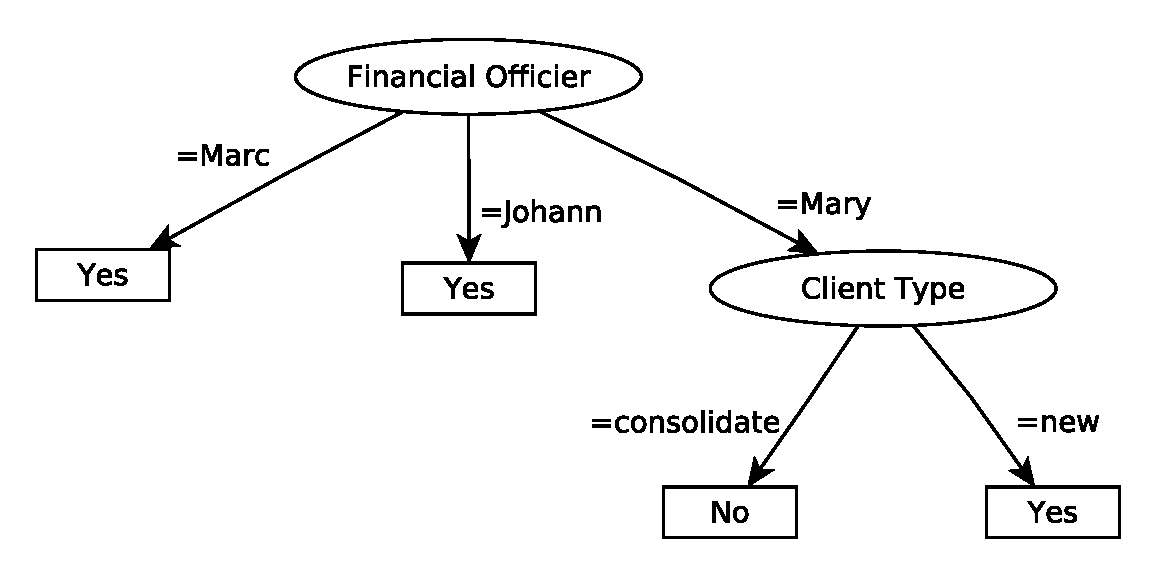
\includegraphics[width=210pt,height=100pt]
{./items/Sales_tree.pdf}
\caption{Decision tree for the conformance analysis.}
\label{salesDecTree}
\end{figure}

The results of the conformance checking enable the use of 
existing machine learning  tools, allowing us to mine the decision tree of Figure~\ref{salesDecTree} as classification model for the sale process.
The resulting decision tree describes a data pattern in correspondence to which a process instance could present conformance errors: order managed by the sales manager \emph{Mary} and received from consolidate clients of the organization may not respect the standard sale procedure. 

From the analysis done for the sale process based on both classification and log replay results, a new scenario of the  sale procedure has emerged: orders done by the consolidate clients of the organization are not checked from a financial point of view. This fact can be accepted as a valid  behavior in a sale procedure, and consequently an extension of the business process model is needed to include the new scenario (\emph{model extension activity}). Alternatively, the misbehaving scenario can be considered as an anomaly in the sale procedure. In this case, since the analysis provides accurate information about the conformance error, corrective measures can be taken in order to prevent such errors in the future.

The classifier constructed with this approach can be used also in a predictive way. Given a trace recording a process execution the decision tree can be used to predict the conformance result. This brings an advantage in terms of the time required by the analysis, since the replay of a process instance  takes more time than its  classification using a decision tree. Moreover, it is worth noting that whenever the set of attributes needed for the classification is  known before the completion of a process execution, the non-conformances predicted by the decision tree can be used to  promptly alert the stakeholders and activate proper countermeasures. 

\subsection{Extension of the approach to Performance Analysis}\label{ClassPerf}
Performance analysis of a process can be carried exploiting log replay. Since an event log contains timestamps, during the replay of a trace it is possible to compute (for each place of the Petri net model) some performance measures such as: \emph{synchronization time} (i.e. time interval between arrival of a token in the place and enabling of a transition in the post-set of the place), \emph{sejour time} (i.e. the time interval between arrival and departure of tokens) and \emph{waiting time} (i.e. the time interval between enabling of a transition in the post-set of the place and token departure).

Performing an analysis based on the measures computed by log replay gives just a \emph{quantitative} information about the process performance. In order to understand the \emph{causes} of performance anomalies that can affect the process behavior, one can explore the process data. Discovering how data attribute can influence process performance provides useful information in analyzing and optimizing the process services. For example, discovering data patterns in correspondence to which some activities need more time for completion than others, helps in making decisions about resources distribution to the process activities or in scheduling activities. In addition to the completion time, one could analyze a process under more complex performance metrics such as the synchronization time. A process with parallel branches and synchronizations can present bottleneck activities that lead to increase the execution time of other activities and consequently the completion time of the entire process. To find out the possible data influences on synchronization time, the approach presented in Section~\ref{ClassConformance} for conformance analysis through classification can be easily extended to performance analysis. For example, a classification problem can be formulated for each synchronization point of the process. In this way, the classifier obtained in correspondence to a synchronization point classifies the process instances based on their attribute value and regarding the synchronization time of the point taken into exam. 

\begin{comment}
\begin{table}[!h]
\scriptsize
\centering
\begin{tabular}{|p{1cm}|p{1cm}|p{1,5cm}|p{1cm}|p{1,3cm}|p{1,4cm}|p{1,1cm}|p{1,2cm}|p{1,5cm}|}
\hline OrdIde & CltIde & CltType & SalMan & FinOff & WrhsMan & Supplier & OrdResut & Synch\\
\hline
1 & 20 & consolidate & Marco & Alessandro & Alex & Gianni & positive & high\_wareh.\\
\hline
2 & 15 & new & Anna & Mario & Alessio & Mario & positive & normal\\
\hline
3 & 10 &consolidate & Maria & Roberto & Alessio & Mario & negative & normal\\
\hline
2 & 15 & new & Anna & Mario & Roberto & Gianni & positive & high\_wareh.\\
\hline
... & ... & ... & ... & ... & ... & ... & .... & .... \\
\hline
\end{tabular}
\caption{Dataset for the performance analysis.}
\label{tab:SaleDataPerf}
\end{table}
\normalsize

To discover how the process data may influence its performance in term of synchronization time, a classification problem is formulated for each synchronization point of the process. In this way, the model obtained in correspondence to a synchronization point classifies the process instances based on their attribute value and regarding the synchronization time of the point taken into exam. For the sales process presented in Section~\ref{example}, a single point of synchronization is identified. In fact, the Petri net in Figure~\ref{pnet} has two parallel branches, one for the financial activity and the other for the warehouse activities. We are interested in analyzing the synchronization between these branches. Indeed, the synchronization time of interest is measured in correspondence to the places $p(8)$ and $p(10)$: $tsc(p8)$, $tsc(p10)$ which are computed by the log replay algorithm as explained in Section~\ref{Background}.

To formulate the classification problem the dataset is extracted from the event log, whereas the target attribute is one of the log replay performance results. The target must be something that characterizes the performance in term of synchronization. An idea can be to simply consider the difference between synchronization time of $p8$ and $p10$: $tsc(p8) - tsc(p10)$. It should be noted that classification deals with discrete or categorical target attribute. Since the performance metrics, the synchronization time in this case, are expressed as continuous values, a discretization phase is required  during the formulation of the classification problem. Let us choose the attribute target as a categorical attribute: given a threshold $S$, if $|tsc(p8)- tsc(p10)|$ exceeds the value $S$, then the target attribute indicates the branch with the high synchronization time, otherwise the target indicates that the instance presents a normal synchronization time. Therefore, the target attribute can assume three possible values: \emph{high\_financial, high\_warehouse} and \emph{normal}. Based on the process data extracted from the event log and target attribute computed by a discretization of the log replay results, the dataset for the classification problem is built and presented in Table~\ref{tab:SaleDataPerf}. As done for conformance analysis, the dataset is used as input of the classification algorithm that returns the decision tree presented in Figure~\ref{salesPerfDecTree}.

\begin{figure}[h]
\centering
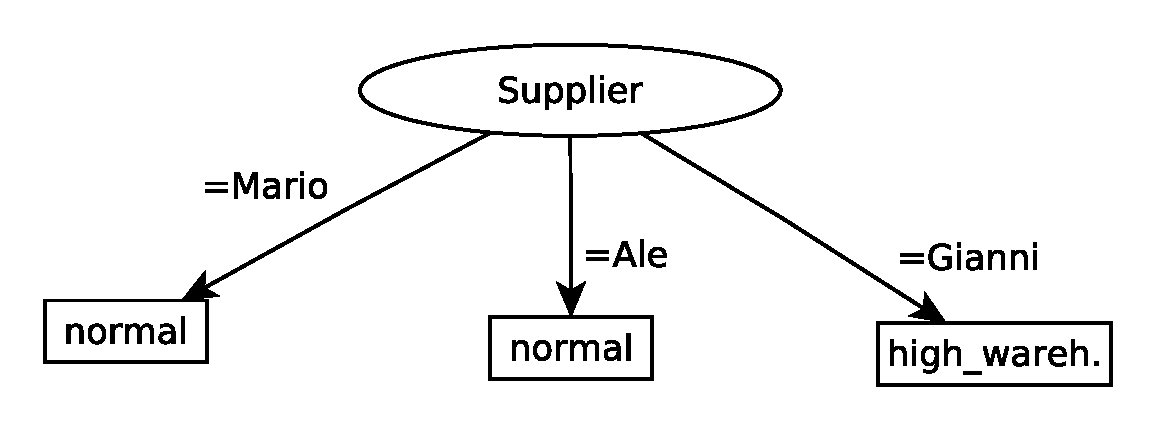
\includegraphics[width=120pt,height=60pt]
{./items/Sales_perf_tree.pdf}
\caption{Decision tree for the performance analysis.}
\label{salesPerfDecTree}
\end{figure}

The decision tree shows that the synchronization time is too high, so not acceptable, for those instances in which the external warehousing is done by the supplier \emph{Gianni}. In other  terms, the rule detected by the decision tree correlates the process performance, measured as the difference of two synchronization times with the external warehousing activities. In this case, the analysis through classification identified such activities as a bottleneck in the \emph{specific case} of the supplier Gianni. This result can be taken as a start point for more investigations that can be done in a \emph{targeted manner} thanks to the pattern identified by the classification analysis. 
\end{comment}

\section{Implementation with ProM}\label{implementation}
In order to experiment with some business process prototypes, the approach presented in this paper has been implemented as a set of plug-ins that integrates \emph{ProM6}~\cite{DBLP:conf/bpm/AalstDGRVW09}, an open-source framework implementing Process Mining tools, and \emph{Weka}~\cite{DBLP:journals/sigkdd/HallFHPRW09}, a data mining framework providing machine learning tools.
We can classify the plug-ins developed in three categories. The first one includes plug-ins for building the dataset needed for the classification:
\begin{itemize}
\item \texttt{Generate Instances with Conformance}: this plug-in takes as input an event log and its conformance results computed by log replay. It returns as output a training set as shown in Table~\ref{tab:SaleData} in the format needed by the Weka classification tool. Note that the plug-in extracts \emph{all} the attributes data recorded in the event log. If necessary, the dataset resulting can be subject to some \emph{feature selection} techniques before using it as a training set for the classification task.  

\item \texttt{Generate Instances to Classify}: given an event log, the plug-in generates a dataset of instances that can be classified using a classification model.
\end{itemize}
The second category includes plug-ins for the classifier generation and utilization as a predictive model:
\begin{itemize}
\item \texttt{Generate Classifier}: given a training set, the plug-in generates a decision tree model using the $J48$ algorithm, an implementation of the algorithm $C4.5$ provided by Weka.
\item \texttt{Classify Instances}: given a set of non-classified instances and a classifier model, this plug-in simply classifies the instances according to the classifier.
\end{itemize}
Finally, the last category includes a set of plug-ins useful for the serialization, deserialization and visualization of the resources used by the previous plug-ins, such as dataset and classifiers. 

Figure \ref{dataflow} represents a data flow diagram that summarizes data dependencies between plug-ins discussed in this section.

\begin{figure}[h]
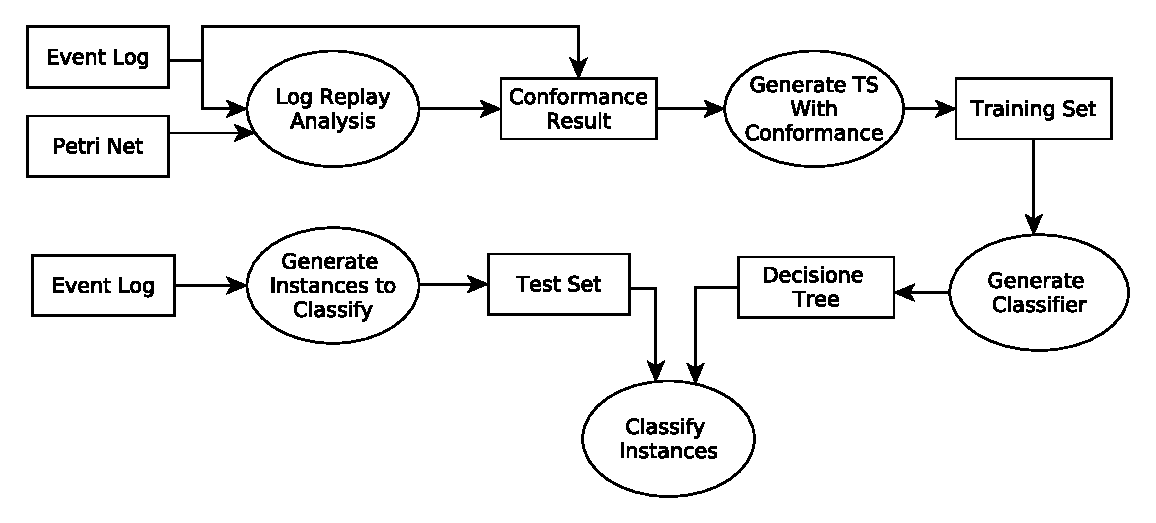
\includegraphics[width=360pt]
{./items/dataflow.pdf}
\caption{Data flow diagram}
\label{dataflow}
\end{figure}



\section{Conclusions and Future Work}

We presented some preliminary results of a research activity aimed at applying machine learning techniques, i.e.~classification algorithms, in the realm of process analysis. The idea is to try to identify some correlation between the data value of certain variables in the process instances of event logs, and the results of conformance checking. A successful identification of such values could allow to predict the conformance result  of an instance during execution.  The same technique was applied to performance checking as well, but only briefly summarized here because of space constraints. The approach is implemented with a combination of plug-ins of the Process Mining framework ProM and of the classification engine Weka. Some guidelines about their use are presented in a concluding section. 
The approach has been successfully tested on synthetic event logs only. An obvious continuation of this work includes experimentations with real event logs: this will allow us to evaluate the scalability of the approach and its robustness in presence of noise.


Classification techniques in the Process Mining field have already been explored in~\cite{DBLP:conf/bpm/RozinatA06} and more recently in~\cite{DBLP:conf/sac/LeoniA13}. In those papers the  idea is to  explore how data influences the case routing of process flow execution, by assigning a classification problem with each decision point in the model. In particular,~\cite{DBLP:conf/sac/LeoniA13} improves significantly the results of~\cite{DBLP:conf/bpm/RozinatA06} by exploiting some recently developed \emph{alignment techniques} between process instances and the process model. We intend to explore how far these techniques can be applied fruitfully in our framework as well.


\addcontentsline{toc}{chapter}{Bibliography} 
\bibliography{biblio}
\bibliographystyle{abbrv} 

\end{document}

